% Template:     Tesis LaTeX
% Documento:    Archivo de ejemplo
% Versión:      3.4.2 (07/02/2025)
% Codificación: UTF-8
%
% Autor: Pablo Pizarro R.
%        pablo@ppizarror.com
%
% Manual template: [https://latex.ppizarror.com/tesis]
% Licencia MIT:    [https://opensource.org/licenses/MIT]

% ------------------------------------------------------------------------------
% NUEVO CAPÍTULO
% ------------------------------------------------------------------------------
% A diferencia de Template-Informe, Template-Tesis requiere el uso de capítulos; las secciones, subsecciones, etc son parte de un capítulo. Se recomienda el uso de un capítulo en un archivo distinto
\chapter{Introducción}

\section{SMBH background}

\lipsum[4]

% SUB-SECCIÓN
% Las sub-secciones se inician con \subsection, si se quiere una sub-sección
% sin número se pueden usar las funciones \subsectionanum (nuevo subtítulo sin
% numeración) o la función \subsectionanumnoi para crear el mismo subtítulo sin
% numerar y sin aparecer en el índice
\subsection{Una breve introducción}
	
	Este es un párrafo, puede contener múltiples \quotes{Expresiones} así como fórmulas o referencias\footnote{Las referencias se hacen utilizando la expresión \texttt{\textbackslash label}\{etiqueta\}.} como \eqref{eqn:identidad-imposible}. A continuación se muestra un ejemplo de inserción de imágenes (como la Figura \ref{img:testimage}) con el comando \href{https://latex.ppizarror.com/informe.html#hlp-imagen}{\textbackslash insertimage}:

	% Esta instrucción, añadida en la v1.1.0 permite cambiar el título de cada
	% objeto en el índice de cada objeto. Este título es solo válido hasta el
	% primer objeto que lo llame, luego este se restablecerá. Por mientras solo
	% se ofrece compatibilidad para las funciones de imágenes. Los entornos como
	% images o sourcecode aún no tienen compatibilidad
	\setindexcaption{Título de la imagen en el índice.}
		
	% Para insertar una imagen se puede usar la función \insertimage la cual
	% toma un primer parámetro opcional para definir una etiqueta (dentro de
	% los corchetes), luego toma la dirección de la imagen, sus parámetros
	% (en este caso se definió la escala de 0.19) y una leyenda opcional
	\insertimage[\label{img:testimage}]{ejemplos/test-image.png}{scale=0.19}{Where are you? de \quotes{Internet}.}

	A continuación\footnote{Como se puede observar las funciones \texttt{\textbackslash insert...} añaden un párrafo automáticamente.} se muestra un ejemplo de inserción de ecuaciones simples con el comando \href{https://latex.ppizarror.com/informe.html#hlp-formulae}{\textbackslash insertequation}:

	% Se inserta una ecuación, el primer parámetro entre [] es opcional
	% (permite identificar con una etiqueta para poder referenciarlo después
	% con \ref), seguido de aquello se escribe la ecuación en modo bruto sin signos $
	\insertequation[\label{eqn:identidad-imposible}]{\pow{a}{k}=\pow{b}{k}+\pow{c}{k} \quad \forall k>2}

	% Notar que no se requiere añadir un salto de línea después de insertar una imagen
	Este template ha sido diseñado para que sea completamente compatible con editores \LaTeX\ para escritorio y de manera online\scite{overleaf}. La compilación es realizada siempre usando las últimas versiones de las librerías, además se incluyen los parches oficiales para corregir eventuales \textit{warnings}. \\

	Este es un nuevo párrafo. Para crear un nuevo párrafo basta con usar \textbackslash\textbackslash\ en el anterior, lo que fuerza una nueva línea. También se insertar un nuevo párrafo con el comando \texttt{\textbackslash newp} si el compilador de latex arroja una alerta del tipo \textit{Underfull \textbackslash hbox (badness 10000) in paragraph at lines ...} \\

	\lipsum[4] \\

	\lipsum[11]

\section{Aims and objectives}

También puedes usar tablas, ¡Crearlas es muy fácil!. Puedes usar el plugin \href{https://www.ctan.org/tex-archive/support/excel2latex}{Excel2Latex} \cite{excel2latex} de Excel para convertir las tablas a \LaTeX\xspace o bien utilizar el \quotes{creador de tablas online} \cite{tablesgenerator}.

% Tabla generada con el plugin Excel2Latex
\begin{table}[H] % Importante el H
	\centering
	\caption{Ejemplo de tablas.}
	\begin{tabular}{ccc}
		\hline
		\textbf{Columna 1} & \textbf{Columna 2} & \textbf{Columna 3} \bigstrut\\
		\hline
		$\omega$ & $\nu$ & $\delta$ \bigstrut[t]\\
		$\Phi$ & $\Theta$ & $\varSigma$ \\
		$\R$ & $\E$ & $\psi$ \\
		\hline
	\end{tabular}
	\label{tab:tabla-1}
\end{table}

% Tabla generada con el plugin Excel2Latex
\enabletablerowcolor
\begin{table}[H]
	\centering
	\caption{Ejemplo de tablas con colores de filas.}
	\begin{tabular}{ccccc}
		\rowcolor[rgb]{ .749,  .749,  .749} \textbf{Valor A} & \textbf{Valor B} & \textbf{Valor C} & \multicolumn{2}{c}{\textbf{Valor Esperado}} \\
		1     & a     & $3x$  & \multicolumn{2}{c}{Cumple} \\
		2     & b     & $6x$  & \multicolumn{2}{c}{No cumple} \\
		3     & c     & $3x+y$ & \multicolumn{2}{c}{Quizás} \\
		4     & d     & $5\sin x$ & \multicolumn{2}{c}{No} \\
		5     & e     & $0$ & \multicolumn{2}{c}{Sí} \\
	\end{tabular}
\end{table}
\disabletablerowcolor
	
\section{Previous work}

El template por defecto está configurado para trabajar con citas de la librería \href{https://www.ctan.org/pkg/natbib}{natbib}, y se configuró al estilo \textit{ieeetr}. Puedes usar otros estilos cambiando la configuración \texttt{\textbackslash natbibrefstyle} si es que usas natbib. También se da soporte a las librerías \textbf{bibtex} y \textbf{apacite}, para ello puedes cambiar la configuración \texttt{\textbackslash stylecitereferences}. Una completa guía de estilos la puedes consultar en \url{https://latex.ppizarror.com/doc/bibstylescompared.pdf}. \\

A continuación se detallan algunos links de ayuda para el uso de las referencias:

\begin{itemize}
    \item \href{https://www.bibtex.com/bibliography-styles-numeric-square-brackets}{Galería de estilos numéricos por corchetes}
    \item \href{https://www.bibtex.com/bibliography-styles-author-date}{Galería de estilos por autor/fecha}
    \item \href{https://latex.ppizarror.com/res/guia_basica_referencias_mendeley_v3.pdf}{Guía básica referencias Mendeley}
    \item \href{https://latex.ppizarror.com/doc/bibstylescompared.pdf}{Guía completa de estilos}
\end{itemize}


% ------------------------------------------------------------------------------
% NUEVO CAPÍTULO
% ------------------------------------------------------------------------------
\chapter{Mathematical model}
\section{density criterion}
\section{Stars and gas in equilibrium}

\chapter{A method for coupling gas and stars}

In this work, we investigate the effect of gas in the process of seeds for SMBH formation. In contrast with other works, we do not take into account gas accretion by stars, since we are interested in the gravitational effect of gas over stars and vice versa.

We need, in principle, three codes: one for the stars, one for the gas and a coupling code that make gravitational interactions between gas and stars.

\begin{figure}[h]
	\centering
	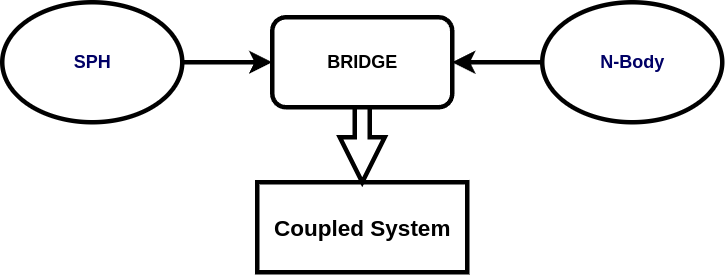
\includegraphics[width=0.8\textwidth]{Esquemas/Codes_scheme.png} % Ruta relativa
	\caption{Codes scheme}
	\label{img:codes_scheme}
\end{figure}

The N-Body and SPH codes are used through the AMUSE interface, and are coupling with an external code.


\section{N-body code: Ph4}

The proposed scenarios presented in (referencia a capitulo) require the modeling of dense stellar clusters. And as we need to consider close encounters and collisions, is necessary a precise code.

We use the PH4 code from the AMUSE interface. In the present section, we include a description of the code, as some external routines.

\subsection{Hermite integrator}

The Ph4 code uses an fourth-order Hermite integrator \cite{makino1992hermite} for calculating the position and velocities of stars due to gravity. This is a predictor-corrector method.

The fourth-order Hermite scheme is based in a precise calculation of the individual time step. Considering the particle $i$ with own time $t_i$, time step $\Delta t_i$, position $x_i$, velocity $v_i$, acceleration $a_i$ and jerk $\dot{a_i}$, calculated at time $t_i$. The algorithm of  integration process proceeds as:

\begin{enumerate}
	\item Select the particle with minimum $t_i + \Delta t_i$. Set the global time as $t=t_i + \Delta t_i$.
	\item Calculate the predicted positions ($x_p$) and velocities ($v_p$) for all particles, using the actual values for $x$, $v$, $a$, $\dot{a}$. 
	\item Calculate the acceleration ($a_i$) and jerk ($\dot{a_i}$) for particle $i$ at time $t_i + \Delta t_i$ using the predicted positions and velocities.
	\item Calculate the second and third time derivative of acceleration ($a_i^{(2)}$ and $a_i^{(3)}$), using an Hermite interpolation.
	\item Add the corrections to position and velocities of particle $i$. Calculate and update the time step $t_i$.
	\item Repeat the algorithm.
\end{enumerate}





\subsection{Block time steps}
\subsection{Collisions and mergers}
\subsection{Escaping stars}

\section{Smoothed particles hydrodynamics: Fi}
\section{Coupling strategy: Bridge}

\chapter{Results and analysis}

\chapter{El desarrollo de la tesis}

\section{Aquí una nueva sección}

\subsection{Haciendo una tesis como un profesional}

	% Se inserta una imagen flotante en la izquierda del documento con
	% \insertimageleft, al igual que las demás funciones, el primer parámetro
	% es opcional, luego viene la ubicación de la imagen, seguido de la escala
	% (un 27% del ancho de página) y por último su leyenda. Para insertar una
	% imagen flotante en la derecha se utiliza \insertimageright usando los
	% mismos parámetros
	\insertimageleft[\label{img:imagen-izquierda}]{ejemplos/test-image-wrap}{0.27}{Apolo flotando a la izquierda.}

	~ \lipsum[6] \newp

	% Párrafos de ejemplo
	~ \lipsum[115]

	% Agrega una ecuación con leyenda
	\insertequationcaptioned[\label{eqn:formulasinsentido}]{\int_{a}^{b} f(x) \dd{x} = \fracnpartial{f(x)}{x}{\eta} \cdotp \textstyle \sum_{x=a}^{b} f(x)\cancelto{1+\frac{\epsilon}{k}}{\bigp{1+\Delta x}}}{Ecuación sin sentido.}

	% Inserta una definición
	\begin{defn}[ver \cite{einstein}]
		Definición definitiva
		$$\frac{d}{dx}\int_a^xf(y)dy=f(x)$$
	\end{defn}

	\lipsum[115]

	% Inserta un subtítulo sin número
	\subsection{Otros párrafos más normales}

	% Párrafos
	\lipsum[7]

	% Se inserta una ecuación larga con el entorno gathered (1 solo número de ecuación)
	\insertgathered[\label{eqn:eqn-larga}]{
		\lpow{\Lambda}{f} = \frac{L\cdot f}{W} \cdot \frac{\pow{\lpow{Q}{e}}{2}}{8 \pow{\pi}{2} \pow{W}{4} g} + \sum_{i=1}^{l} \frac{f \cdot \bigp{M - d}}{l \cdot W} \cdot \underequal{\frac{\pow{\bigp{\lpow{Q}{e}- i\cdot Q}}{2}}{8 \pow{\pi}{2} \pow{W}{4} g}}{\sim \A}\\
			Q_e = 2.5Q \cdot \int_{0}^{e} V(x) \dd{x} + \aasin{\biggp{1+\frac{1}{1-e}}}
	}

	% Nuevo párrafo
	\lipsum[4]

	% Se inserta un multicols, con esto se pueden escribir párrafos en varias columnas
	\begin{multicols}{2}

		% Párrafo 1
		\lipsum[4]

		% Ecuación encerrada en una caja
		\insertequation[]{ \boxed{f(x) = \fracdpartial{u}{t}} }

		% Párrafo 2 del multicols
		\lipsum[2-3]

	\end{multicols}

\subsection{Ejemplos de inserción de código fuente}

	% A continuación se crea una función auxiliar, esta es una herramienta
	% extremadamente importante y muy útil. Esta función de ejemplo toma dos
	% parámetros, uno es el lenguaje del código fuente, el segundo el
	% identificador en el manual
	\newcommand{\insertsrcmanual}[2]{\href{https://latex.ppizarror.com/informe.html?srctype=#1\#hlp-srccode}{#2}}

	El template permite la inserción de los siguientes lenguajes de programación de forma nativa: \insertsrcmanual{abap}{ABAP}, \insertsrcmanual{ada}{Ada}, \insertsrcmanual{assemblerx64}{Assembler x64}, \insertsrcmanual{assemblerx86}{Assembler x86[masm]}, \insertsrcmanual{awk}{Awk}, \insertsrcmanual{bash}{Bash}, \insertsrcmanual{basic}{Basic}, \insertsrcmanual{c}{C}, \insertsrcmanual{caml}{Caml}, \insertsrcmanual{cmake}{CMake}, \insertsrcmanual{cobol}{Cobol}, \insertsrcmanual{cpp}{C++}, \insertsrcmanual{csharp}{C\#}, \insertsrcmanual{css}{CSS}, \insertsrcmanual{csv}{CSV}, \insertsrcmanual{cuda}{CUDA}, \insertsrcmanual{dart}{Dart}, \insertsrcmanual{docker}{Docker}, \insertsrcmanual{elisp}{Elisp}, \insertsrcmanual{elixir}{Elixir}, \insertsrcmanual{erlang}{Erlang}, \insertsrcmanual{fortran}{Fortran}, \insertsrcmanual{fsharp}{F\#}, \insertsrcmanual{glsl}{GLSL}, \insertsrcmanual{gnuplot}{Gnuplot}, \insertsrcmanual{go}{Go}, \insertsrcmanual{haskell}{Haskell}, \insertsrcmanual{html}{HTML}, \insertsrcmanual{ini}{INI}, \insertsrcmanual{java}{Java}, \insertsrcmanual{javascript}{Javascript}, \insertsrcmanual{json}{JSON}, \insertsrcmanual{julia}{Julia}, \insertsrcmanual{kotlin}{Kotlin}, \insertsrcmanual{latex}{LaTeX}, \insertsrcmanual{lisp}{Lisp}, \insertsrcmanual{llvm}{LLVM}, \insertsrcmanual{lua}{Lua}, \insertsrcmanual{make}{Make}, \insertsrcmanual{maple}{Maple}, \insertsrcmanual{mathematica}{Mathematica}, \insertsrcmanual{matlab}{Matlab}, \insertsrcmanual{mercury}{Mercury}, \insertsrcmanual{modula2}{Modula-2}, \insertsrcmanual{objectivec}{Objective-C}, \insertsrcmanual{octave}{Octave}, \insertsrcmanual{opencl}{OpenCL}, \insertsrcmanual{opensees}{OpenSees}, \insertsrcmanual{pascal}{Pascal}, \insertsrcmanual{perl}{Perl}, \insertsrcmanual{php}{PHP}, \insertsrcmanual{plaintext}{Texto plano}, \insertsrcmanual{postscript}{PostScript}, \insertsrcmanual{powershell}{Powershell}, \insertsrcmanual{prolog}{Prolog}, \insertsrcmanual{promela}{Promela}, \insertsrcmanual{pseudocode}{Pseudocódigo}, \insertsrcmanual{python}{Python}, \insertsrcmanual{qsharp}{Q\#}, \insertsrcmanual{r}{R}, \insertsrcmanual{racket}{Racket}, \insertsrcmanual{reil}{Reil}, \insertsrcmanual{ruby}{Ruby}, \insertsrcmanual{rust}{Rust}, \insertsrcmanual{scala}{Scala}, \insertsrcmanual{scheme}{Scheme}, \insertsrcmanual{scilab}{Scilab}, \insertsrcmanual{simula}{Simula}, \insertsrcmanual{sparql}{SPARQL}, \insertsrcmanual{sql}{SQL}, \insertsrcmanual{swift}{Swift}, \insertsrcmanual{tcl}{TCL}, \insertsrcmanual{vbscript}{VBScript}, \insertsrcmanual{verilog}{Verilog}, \insertsrcmanual{vhdl}{VHDL} y \insertsrcmanual{xml}{XML}. \\
		
	Para insertar un código fuente se debe usar el entorno \texttt{sourcecode}, o el entorno \texttt{sourcecodep} si es que se quiere utilizar parámetros adicionales. A continuación se presenta un ejemplo de inserción de código fuente en Python (Código \ref{codigo-python}), Java y Matlab:

% Se define el lenguaje del código. Cuidado: Los códigos en LaTeX son sensibles
% a las tabulaciones y espacios en blanco
\begin{sourcecode}[\label{codigo-python}]{python}{Ejemplo en Python.}
import numpy as np
def incmatrix(genl1, genl2):
	m = len(genl1)
	n = len(genl2)
	M = None # Comentario 1
	VT = np.zeros((n*m, 1), int) # Comentario 2
\end{sourcecode}

\begin{sourcecode}[]{java}{Ejemplo en Java.}
import java.io.IOException;
import javax.servlet.*;

public class Hola extends GenericServlet { // Hola mundo
	public void service(ServletRequest request, ServletResponse response)
	throws ServletException, IOException{
		response.setContentType("text/html");
		PrintWriter pw = response.getWriter();
		pw.println("Hola, mundo!");
	}
}
\end{sourcecode}

\begin{sourcecode}{matlab}{Ejemplo en Matlab.}
% Se crea gráfico
f = figure(1);
title('Espectro de pulso de desplazamiento');

for j = 1:length(BETA)
	fad = ones(1, NDATOS); % Arreglo para el FAD
	for i = 1:NDATOS
		[t, u_t, ~, ~] = main(BETA(j), r(i), M, K, F0, 0);
		fad(i) = max(abs(u_t)) / uf0;
	end
end
\end{sourcecode}

% SUB-SECCIÓN
\subsection{Agregando múltiples imágenes}

	El template ofrece el entorno \href{https://latex.ppizarror.com/informe.html#hlp-images}{images} que permite insertar múltiples imágenes de una manera muy sencilla. Para crear imágenes múltiples se deben usar las siguientes instrucciones:

\begin{sourcecode}{latex}{}
\begin{images}[\label{imagenmultiple}]{Ejemplo de imagen múltiple.}
	\addimage[\label{ciudadfoto}]{ejemplos/test-image}{width=6.5cm}{Ciudad}
	\addimageanum{ejemplos/test-image-wrap}{height=4cm}
	\imagesnewline
	\addimage{ejemplos/test-image}{width=11cm}{Ciudad más grande}
\end{images}
\end{sourcecode}

	Obteniendo así:

	\begin{images}{Ejemplo de imagen múltiple.}
		\addimage{ejemplos/test-image}{width=6.5cm}{Ciudad}
		\addimageanum{ejemplos/test-image-wrap}{height=4cm}
		\imagesnewline
		\addimage{ejemplos/test-image}{width=11cm}{Ciudad más grande}
	\end{images}

% Inserta una sección sin número
\clearpage
\sectionanum{Más ejemplos}

% Inserta un subtítulo sin número
\subsectionanum{Listas y Enumeraciones}

	Hacer listas enumeradas con \LaTeX\ es muy fácil con el template\footnote{También puedes revisar el manual de las enumeraciones en \url{https://latex.ppizarror.com/doc/enumitem.pdf}.}, también puedes revisar el manual \cite{template}, para ello debes usar el comando \texttt{\textbackslash begin\{enumerate\}}, cada elemento comienza por \texttt{\textbackslash item}, resultando así:

	\begin{enumerate}
		\item Grecia
		\item Abracadabra
		\item Manzanas
	\end{enumerate}

	También se puede cambiar el tipo de enumeración, se pueden usar letras, números romanos, entre otros. Esto se logra cambiando el \textbf{label} del objeto \texttt{enumerate}. A continuación se muestra un ejemplo usando letras con el estilo \texttt{\textbackslash alph}\footnote{Con \texttt{\textbackslash Alph} las letras aparecen en mayúscula.}, números romanos con \texttt{\textbackslash roman}\footnote{Con \texttt{\textbackslash Roman} los números romanos salen en mayúscula.} o números griegos con \texttt{\textbackslash greek}\footnote{Una característica propia del template, con \texttt{\textbackslash Greek} las letras griegas están escritas en mayúscula.}:

	\begin{multicols}{3}
		\begin{enumeratebf}[label=\alph*) ] % Fuente en negrita
			\item Peras
			\item Manzanas
			\item Naranjas
		\end{enumeratebf}

		\begin{enumerate}[label=\roman*) ]
			\item Rojo
			\item Café
			\item Morado
		\end{enumerate}
		
		\begin{enumerate}[label=\greek*) ]
			\item Matemáticas
			\item Lenguaje
			\item Filosofía
		\end{enumerate}
	\end{multicols}

	Para hacer listas sin numerar con \LaTeX\ hay que usar el comando \texttt{\textbackslash begin\{itemize\}}, cada elemento empieza por \texttt{\textbackslash item}, resultando:

	\begin{multicols}{3}
		\begin{itemize}[label={--}]
			\item Peras
			\item Manzanas
			\item Naranjas
		\end{itemize}

		\begin{enumerate}[label={*}]
			\item Rojo
			\item Café
			\item Morado
		\end{enumerate}

		\begin{itemize}
			\item Árboles
			\item Pasto
			\item Flores
		\end{itemize}
	\end{multicols}


% ------------------------------------------------------------------------------
% NUEVO CAPÍTULO
% ------------------------------------------------------------------------------
\chapter{Conclusions}

\lipsum[1] \\

\lipsum[2]


% ------------------------------------------------------------------------------
% REFERENCIAS, revisar configuración \stylecitereferences
% ------------------------------------------------------------------------------
\bibliography{library}


% ------------------------------------------------------------------------------
% ANEXO
% Existe adicionalmente el entorno \begin{appendixd} que permite insertar
% \chapter y el entorno \begin{appendixdtitle}[style1] (4 estilos diferentes),
% el cual acepta \chapter y escribe el título de anexos encima
% ------------------------------------------------------------------------------
\begin{appendixs}
	
	\section{Cálculos realizados}

	\subsection{Metodología}
	\lipsum[1-2]

	% Imagen, se numerará automáticamente con la letra del anexo según
	% la configuración \appendixindepobjnum
	\insertimage[\label{img:anexo-2}]{ejemplos/test-image.png}{scale=0.25}{Imagen en anexo.}

	\subsection{Resultados}
	\lipsum[10]

	% Tablas
	\enabletablerowcolor[2] % Activa el color de celda
	\begin{table}[H]
		\begin{threeparttable}
		\centering
		\caption{Tabla de cálculo.}
		\begin{tabular}{cccC{4cm}}
			\hline
			\textbf{Elemento} & $\epsilon_i$ & \textbf{Valor} & \textbf{Descripción} \bigstrut \\
			\hline
			A     & 10    & 3,14$\pi$ & Valor muy interesante\tnote{a} \\
			B     & 20    & 6 & Segundo elemento \\
			C     & 30    & 7 & Tercer elemento\tnote{1} \\
			D     & 150    & 10 & Sin descripción \\
			E     & 0    & 0 & Cero \\
			\hline
			\end{tabular}
		\begin{tablenotes}
			\item[a] Este elemento tiene una descripción debajo de la tabla
			\item[1] Más comentarios
		\end{tablenotes}
		\end{threeparttable}
		\label{tab:anexo-1}
	\end{table}
	\disabletablerowcolor % Desactiva el color de celda

\end{appendixs}